%credits K. Κουνής, I. Στεφανίδου 
%refactoring : K.Draziotis (drazioti@gmail.com
%Licence CC_BY_SA

\documentclass[12pt]{article}
\usepackage{helvet} 
\usepackage{amsmath}
\usepackage{titlesec}
\usepackage{lipsum}
\usepackage{textcomp}
\usepackage{graphicx}
\usepackage{float}
\usepackage{listings}
\usepackage{xcolor}
\graphicspath{{images/}}


\usepackage{listings}
\usepackage{xcolor}

\definecolor{codegreen}{rgb}{0,0.6,0}
\definecolor{codegray}{rgb}{0.5,0.5,0.5}
\definecolor{codepurple}{rgb}{0.58,0,0.82}
\definecolor{backcolour}{rgb}{0.95,0.95,0.92}

\lstdefinestyle{mystyle}{
    backgroundcolor=\color{backcolour},   
    commentstyle=\color{codegreen},
    keywordstyle=\color{magenta},
    numberstyle=\tiny\color{codegray},
    stringstyle=\color{codepurple},
    basicstyle=\ttfamily\footnotesize,
    breakatwhitespace=false,         
    breaklines=true,                 
    captionpos=b,                    
    keepspaces=true,                 
    numbers=left,                    
    numbersep=5pt,                  
    showspaces=false,                
    showstringspaces=false,
    showtabs=false,                  
    tabsize=2
}
\lstset{style=mystyle}

\lstset{
    basicstyle=\ttfamily,
    breaklines=true,
    inputencoding=utf8,
    extendedchars=true,
    language=bash,
    showstringspaces=false,
    keywordstyle=\color{blue},
    commentstyle=\color{gray},
    stringstyle=\color{red},
}

\titleformat{\section}[display]
          {\clearpage\vspace*{50pt}%
          \normalfont\huge\bfseries}%
          {{\Kappa}E{\Phi}A{\Lambda}AIO \thesection}%
          {20pt}%
          {\Huge}%
          [\vspace{40pt}]

\usepackage[algosection,commentsnumbered,ruled,vlined]{algorithm2e}
\NoCaptionOfAlgo
\usepackage{chemarrow}
\newcommand\aug{\fboxsep=-\fboxrule\!\!\!\fbox{\strut}\!\!\!}
\usepackage{graphicx}
\usepackage{gfsdidot}
\usepackage[LGR,T1]{fontenc}
\usepackage[utf8]{inputenc}
\usepackage[english,greek]{babel} % και για τις δυο γλώσσες
\usepackage{alphabeta}
\usepackage[hidelinks]{hyperref}
\usepackage{hyperref}
\usepackage{makeidx}
\usepackage{enumerate}
\usepackage{enumitem}
\usepackage{systeme}
\usepackage{algorithmic}
\usepackage{comment}

% TEXT FORMATTING
% set spacing between lines (διάστιχο)
\usepackage{setspace}
\setstretch{1.5}
% package to customize chapters, sections and subsections style
\usepackage{titlesec}
% chapter title appearance format
\titleformat{\chapter}[display]
{\bfseries\huge}{\chaptertitlename\space\thechapter}{16pt}{}
% https://www.sharelatex.com/learn/Sections_and_chapters
\titlespacing{\chapter}{0pc}{1.5ex plus .1ex minus .2ex}{5pc}
% section title appearance format
\titleformat{\section}
{\bfseries\large}{\thesection}{14pt}{}
% subsection title appearance format
\titleformat{\subsection}
{\bfseries\normalsize}{\thesubsection}{12pt}{}
% set margins
\usepackage{geometry}
\geometry{left=3cm, right=2cm, top=4cm, bottom=3cm}
\usepackage{graphicx}
% put images in images path
\graphicspath{{images/}}
\usepackage{setspace}

% Caption customization
% use this package to set appearance for captions
\usepackage{caption}
% caption size for figures 10pt
\captionsetup[figure]{font=footnotesize,labelfont=footnotesize}
% caption size for tables 10pt and underlined
\usepackage[normalem]{ulem} % Package for underlining
\DeclareCaptionLabelFormat{label_format}{\uline{#1~#2}} % underline label
\DeclareCaptionTextFormat{text_format}{\uline{#1}} % underline text
\DeclareCaptionLabelSeparator{separator_format}{\uline{:~}} % underline separator
\captionsetup[table]{font=normalsize,labelfont=normalsize,labelformat=label_format,textformat=text_format,labelseparator=separator_format}

% use this package to define custom colors
\usepackage{xcolor}

% create colors
\colorlet{punct}{red!60!black}
\definecolor{background}{HTML}{EEEEEE}
\definecolor{delim}{RGB}{20,105,176}
\colorlet{numb}{magenta!60!black}

\usepackage{amsfonts}
\usepackage{amscd}
\usepackage{amssymb}
\newtheorem{algor}{\bf{Algorithm}}[subsection]

\newtheorem{remark}{Remark}[section]
\newtheorem{theorem}{Theorem}[section]
\newtheorem{lemma}[theorem]{Lemma}
\newtheorem{definition}[theorem]{Definition}
\newtheorem{proposition}[theorem]{Proposition}

% use this package to show actual code listings
\usepackage{listings}

% change listings name in caption to Απεικόνιση
\renewcommand{\lstlistingname}{Απεικόνιση}

% change listings name in contents page to Κατάλογος απεικονήσεων
\renewcommand\lstlistlistingname{Κατάλογος απεικονίσεων}

% set custom colorscheme for listings
\lstdefinelanguage{lang1}{
    basicstyle=\normalfont\ttfamily,
    showstringspaces=false,
    breaklines=true,
    frame=lines,
    backgroundcolor=\color{background},
    literate=
     *{0}{{{\color{numb}0}}}{1}
      {1}{{{\color{numb}1}}}{1}
      {2}{{{\color{numb}2}}}{1}
      {3}{{{\color{numb}3}}}{1}
      {4}{{{\color{numb}4}}}{1}
      {5}{{{\color{numb}5}}}{1}
      {6}{{{\color{numb}6}}}{1}
      {7}{{{\color{numb}7}}}{1}
      {8}{{{\color{numb}8}}}{1}
      {9}{{{\color{numb}9}}}{1}
      {:}{{{\color{punct}{:}}}}{1}
      {,}{{{\color{punct}{,}}}}{1}
      {\{}{{{\color{delim}{\{}}}}{1}
      {\}}{{{\color{delim}{\}}}}}{1}
      {[}{{{\color{delim}{[}}}}{1}
      {]}{{{\color{delim}{]}}}}{1},
}

% create command for blank page
\usepackage{afterpage}
\newcommand\blankpage{%
    \null
    \thispagestyle{empty}%
    \addtocounter{page}{-1}%
    \newpage}
    
\definecolor{maroon}{HTML}{AF3235}
% add clickable hyperlinks
\usepackage{hyperref}
\hypersetup{
    colorlinks,
    citecolor=black,
    filecolor=black,
    linkcolor=black,
    urlcolor=black
}

% use fancy header and footer
\usepackage{fancyhdr}
\usepackage{blindtext} 

% Turn on the style
\pagestyle{fancy}

% Clear the header and footer
\fancyhf{}

% Set the right side of the footer to be the page number
\fancyfoot[R]{\thepage}

% set page number appearance to bottom right
\fancypagestyle{plain}{%
    \renewcommand{\headrulewidth}{0pt}
    \fancyhf{}
    \fancyfoot[R]{\thepage}%
}

\newcommand{\HRule}{\rule{\linewidth}{0.5mm}}
\newcommand{\lt}{\latintext}

\begin{document}
\begin{titlepage}

{\LARGE Αριστοτέλειο Πανεπιστήμιο Θεσσαλονίκης}
\begin{center} {\Large Σχολή Θετικών Επιστημών} \end{center}
\begin{figure}[h]
\raggedright
\hspace{90pt}
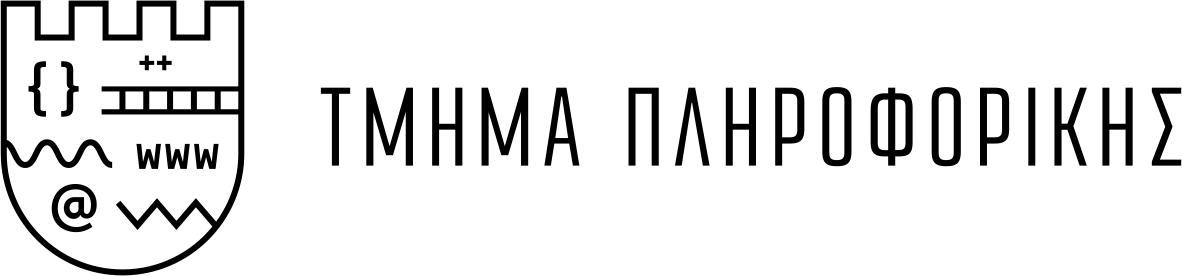
\includegraphics[width=0.5\linewidth]{logo.png}
\end{figure}
\begin{center}

\begin{figure}[h]
\centering 
%\includegraphics[width=0.3\linewidth]{authLogo.png}
\end{figure}
\begin{center}
% leave 2 cm from above text

\HRule \\[0.4cm]
{\huge {\lt{Steepest Descent Optimization \& Advanced Gradient Methods}}}

\HRule \\[0.4cm]
\end{center}

% put this on the bottom
\vfill
\begin{doublespacing}

{\LARGE 
Σπυριδόπουλος Γεώργιος  {\lt{gspyridop@csd.auth.gr}} ΑΕΜ: 4619\\}

\vfill 
{\Large \today}
\end{doublespacing}
\end{center}
\end{titlepage}

\clearpage

\addcontentsline{toc}{section}{Εισαγωγή}
\section*{{\color{maroon}{Εισαγωγή: Η Μέθοδος \lt{Steepest Descent} και το Πρόβλημα Σύγκλισης}}}
\lt{}

Η μέθοδος \lt{Steepest Descent} ή αλλιώς \lt{Gradient Descent} αποτελεί μια βασική τεχνική βελτιστοποίησης για την εύρεση τοπικών ελαχίστων. 

\subsection*{Αλγόριθμος \lt{Steepest Descent}}
\begin{enumerate}
    \item Αρχική πρόβλεψη/διάνυσμα $x_0$ και ορισμός $\epsilon > 0$, $k=0$.
    \item Επαναληπτικό Βήμα:
    \begin{enumerate}[label=\alph*)]
        \item Αν $\|\nabla f(x_k)\| < \epsilon$, τότε ο αλγόριθμος τερματίζει και η προσεγγιστική λύση είναι το $x^*$.
        \item Αλλιώς, υπολογίζουμε την κατεύθυνση καθόδου $p_k = -\nabla f(x_k)$.
        \item Βρίσκουμε το $\alpha_k > 0$ \lt{step-size} που ελαχιστοποιεί τη συνάρτηση $\varphi(\alpha_k) = f(x_k + \alpha_k p_k)$.
        \item Θέτουμε το νέο σημείο $x_{k+1} = x_k + \alpha_k p_k$.
        \item Επαναλαμβάνουμε από το βήμα (α) θέτοντας $k \leftarrow k+1$.
    \end{enumerate}
\end{enumerate}

\textbf{Το Πρόβλημα της Σύγκλισης:} \\
Η πορεία προς το ελάχιστο είναι μία τεθλασμένη γραμμή με μεγάλο αριθμό διαδοχικών ευθύγραμμων τμημάτων τα οποία σχηματίζουν ορθές γωνίες ($90^\circ$) μεταξύ τους, καθιστώντας τη μέθοδο αργή και αναποτελεσματική. Μόνο αν ξεκινήσουμε με ένα αρχικό σημείο $x_0$ τέτοιο ώστε το διάνυσμα προς το $x^*$ να είναι συγγραμμικό του $\nabla f(x_0)$, ο αλγόριθμος τερματίζει σε ένα βήμα.

Μελετώντας την \lt{steepest descent} στην τετραγωνική συνάρτηση $f(x) = \frac{1}{2}x^T Q x - b^T x + c$, υπολογίζουμε πως ισχύει η παρακάτω ανισότητα σφάλματος:
\begin{equation}
\|x_{k+1} - x^*\|_Q^2 \le \left( \frac{\lambda_n - \lambda_1}{\lambda_n + \lambda_1} \right)^2 \|x_k - x^*\|_Q^2
\end{equation}
όπου $\lambda_1, \dots, \lambda_n$ είναι οι ιδιοτιμές του $Q$. Συμπεραίνουμε λοιπόν, πως στην συγκεκριμένη περίπτωση συγκλίνει γραμμικά.

\vspace{1cm}

\section*{{\color{maroon}{Momentum - Heavy-Ball}}}
\subsubsection*{Why Momentum Really Works \cite{goh2017momentum}}
Το άρθρο αναφέρεται στην μέθοδο \lt{momentum} ή αλλίως \lt{heavy-ball} και αναλύει τον ρυθμό σύγκλισής τους στην τετραγωνική συνάρτηση $f(w) = \frac{1}{2}w^T A w - b^T w$, συγκριτικά με την \lt{steepest descent}.

\subsubsection*{Τύπος και σύγκριση}

Στην κλασική \lt{steepest descent}, έχουμε:
\begin{equation}
w^{k+1} = w^k - \alpha \nabla f(w^k)
\end{equation}
ενώ στη μέθοδο \lt{momentum}, εισάγεται η έννοια της μνήμης για να αποτραπούν οι απότομες ταλαντώσεις:
\begin{equation}
z^{k+1} = \beta z^k + \nabla f(w^k) \quad \text{και} \quad w^{k+1} = w^k - \alpha z^{k+1}
\end{equation}

Στην τετραγωνική συνάρτηση η \lt{steepest descent} επιτυγχάνει με βέλτιστο βήμα $\alpha^* = \frac{2}{\lambda_n + \lambda_1}$, ρυθμό σύγκλισης:
\begin{equation}
\text{rate}(\alpha^*) = 1 - \alpha^* \lambda_1 = \frac{\lambda_n/\lambda_1 - 1}{\lambda_n/\lambda_1 + 1} = \frac{\kappa - 1}{\kappa + 1}
\end{equation}
όπου $\kappa = \frac{\lambda_n}{\lambda_1}$ είναι ο δείκτης κατάστασης (\lt{condition number}). Αποδεικνύεται ότι απαιτούνται $k = \mathcal{O}(\kappa)$ επαναλήψεις.

Στο ίδιο πρόβλημα, η μέθοδος \lt{momentum} για βέλτιστα $\alpha$ και $\beta$:
\begin{equation}
\alpha^* = \frac{4}{(\sqrt{\lambda_n} + \sqrt{\lambda_1})^2}, \quad \beta^* = \left( \frac{\sqrt{\lambda_n} - \sqrt{\lambda_1}}{\sqrt{\lambda_n} + \sqrt{\lambda_1}} \right)^2
\end{equation}
έχει ρυθμό σύγκλισης $\rho = \sqrt{\beta^*} = \frac{\sqrt{\kappa} - 1}{\sqrt{\kappa} + 1}$. Έτσι, η πολυπλοκότητα βελτιώνεται σε $\mathcal{O}(\sqrt{\kappa})$.
Ο \lt{Nesterov} απέδειξε πως καμία άλλη μέθοδος στη κλάση των γραμμικών μεθόδων πρώτης τάξης (\lt{linear first order methods}), δεν έχει καλύτερο ρυθμό για τετραγωνικές συναρτήσεις.
Γενικότερα, η μέθοδος \lt{momentum} έχει τον προαναφερόμενο ρυθμό σε τετραγωνικές συναρτήσεις.

\vspace{1cm}

\section*{{\color{maroon}{Nesterov Accelerated Gradient (NAG)}}}

\subsection*{Πρόβλεψη Μετάβασης (NAG - 1983) \cite{ruder2016optimizing}}

Η μέθοδος \lt{NAG}, σε αντίθεση με την \lt{momentum}, προβλέπει την θέση του επόμενου βήματος και έπειτα διορθώνει χρησιμοποιώντας την κλίση στο σημείο το οποίο πιστεύει ότι περίπου θα είναι:
\begin{align}
y^k &= w^k + \beta(w^k - w^{k-1}) \quad (\text{Σημείο πρόβλεψης - \lt{lookahead point}}) \\
w^{k+1} &= w^k - \alpha \nabla f(y^k) \quad (\text{Βήμα διόρθωσης - \lt{correction step}})
\end{align}
Το σημείο $y^k$ είναι η θέση στην οποία η ορμή, χωρίς την κλίση, θα μας πήγαινε.

Η μέθοδος NAG επιτυγχάνει ρυθμό σύγκλισης $\frac{\sqrt{\kappa} - 1}{\sqrt{\kappa} + 1}$ σε όλες τις κυρτές συναρτήσεις, όχι μόνο στην τετραγωνική όπως η μέθοδος \lt{momentum}.

\vspace{1cm}

\section*{{\color{maroon}{Μέθοδοι Κλίσης με Βήμα Δύο Σημείων (Barzilai-Borwein)}}}

\subsection*{\lt{Barzilai-Borwein Method} \cite{barzilai1988two}}

Οι J. Barzilai και J. Borwein πρότειναν μία μέθοδο που το βήμα $\alpha_k$ υπολογίζεται συναρτήσει της τωρινής και της προηγούμενης επανάληψης. Για τις διαφορές των θέσεων και κλίσεων:
\begin{equation}
\Delta x = x_k - x_{k-1}, \quad \Delta g = \nabla f(x_k) - \nabla f(x_{k-1})
\end{equation}
υπάρχουν δύο εναλλακτικές.
\begin{itemize}
    \item \textbf{BB1 (Long-step)}: Ελαχιστοποιεί την ποσότητα $\|\Delta x - \alpha \Delta g\|^2$, δίνοντας τον τύπο:
    \begin{equation}
    \alpha_k = \frac{\langle \Delta x, \Delta x \rangle}{\langle \Delta x, \Delta g \rangle}
    \end{equation}
    
    \item \textbf{BB2 (Short-step)}: Ελαχιστοποιεί την αντίστοιχη ποσότητα για τον αντίστροφο μετασχηματισμό, δίνοντας τον τύπο:
    \begin{equation}
    \alpha_k = \frac{\langle \Delta x, \Delta g \rangle}{\langle \Delta g, \Delta g \rangle}
    \end{equation}
\end{itemize}

Έτσι, για παράδειγμα στην τετραγωνική συνάρτηση, η μέθοδος \lt{BB} έχει πολυπλοκότητα $\mathcal{O}(n)$, λόγω εσωτερικού γινομένου, ενώ η \lt{steepest descent} έχει $\mathcal{O}(n^2)$

\section*{{\color{maroon}{Θεωρητικό Συμπέρασμα}}}

Διαπιστώνεται ότι οι μέθοδοι \lt{Momentum} και \lt{NAG} λειτουργούν αποδοτικότερα για σταθερό και βέλτιστο $\alpha$ (\lt{learning rate}) και $\beta$ (\lt{momentum/memory term}). Αντίθετα, η κλασική \lt{Steepest Descent} και η \lt{Barzilai-Borwein} βασίζονται στο παρόν ή και το παρελθόν για τον υπολογισμό του βήματος,. 

Είναι σημαντικό να τονιστεί πως οι τέσσερις παραπάνω τεχνικές ανήκουν οικογένεια των μεθόδων βελτιστοποίησης \textit{πρώτης τάξης}. Συνεπώς, η κατεύθυνσή τους επηρεάζεται απολύτως και άμεσα από την τωρινή κλίση συνάρτησης. Αποτελεσματικά, για μη-κυρτές (\lt{non-convex}) συναρτήσεις, είναι πιθανό να παγιδευτούν σε τοπικά ελάχιστα καθώς δεν υπάρχει πλήρης εικόνα του χώρου.

\clearpage

\bibliographystyle{unsrt}
\bibliography{bib.bib}

\end{document}